\makeatletter
\def\input@path{{./}{../}{../../}{../../../}{../../../../}{preamble/}{../preamble/}{../../preamble/}{../../../preamble/}}
\makeatother
\input{preamble_exams.tex}

% Local diagram styles use the TikZ libraries already loaded by the project.
\tikzset{cNineDecision/.style={draw,rectangle,minimum size=6mm,inner sep=1pt},
 cNineChance/.style={draw,circle,minimum size=6mm,inner sep=1pt},
 cNineEnd/.style={draw,circle,fill=black,inner sep=1.2pt},
 cNineLabel/.style={font=\small,fill=white,inner sep=2pt}}
\title{Grade 10 -- Term 1\\Decision Trees: Practice Activity (C9)}
\author{}
\date{}
\begin{document}
\maketitle
\setcounter{tocdepth}{1}
\setcounter{secnumdepth}{2}
\phantomsection\label{toc}
\tableofcontents
\section*{Evaluated criteria}
\begin{enumerate}[label=\textbf{C\arabic*},start=9]
\item Builds and solves decision trees by distinguishing decision nodes and chance nodes, assigning probabilities and payoffs, and applying backward induction to identify an optimal strategy.
\end{enumerate}

\section{Introduction}\label{sec:introduction}
\subsection{Reading a decision tree}
A decision tree organises a decision-making problem in chronological order from left to right. It shows available alternatives, uncertain states of nature, and the economic consequences of each possible sequence. Every complete path ends at a \textbf{terminal outcome} with a monetary payoff.
\begin{center}
\begin{tabularx}{\textwidth}{@{}lX@{}}\toprule
Element & Meaning and construction rule\\\midrule
Square: decision node & The decision-maker chooses one outgoing branch. Label branches with alternatives; do not assign probabilities to choices.\\
Circle: chance node & An uncertain event occurs. Label each outgoing branch with a state of nature and its probability. Probabilities must lie in $[0,1]$ and sum to $1$ at that node.\\
Branch & An available action or a possible event. Its position shows when it occurs and which earlier outcomes are known.\\
Filled dot: terminal outcome & The path ends. Write its final net profit beside it, including all costs incurred along that path.\\\bottomrule
\end{tabularx}
\end{center}
Use $A_i$ for alternatives, $S_j$ for states of nature, $P(S_j)$ for probabilities, and $P_{ay}(A_i,S_j)$ for payoffs, as in the earlier activities. Here, all payoffs are \textbf{net profits in thousands of US dollars}, unless a different currency is stated. A payoff of $-10$ means a loss of \$10,000. Do not deduct a cost again if it is already included in a stated net payoff.

\subsection{Backward induction}
Start at the terminal outcomes and work \textbf{from right to left}. Write a value $V$ beside each node:
\[
V(\text{chance node})=EMV=\sum_j P(S_j)V_j,
\qquad V(\text{decision node})=\max\{V_1,V_2,\ldots\}.
\]
Here $V_j$ is the payoff or already calculated value reached by branch $j$. At a chance node, take a probability-weighted average. At a decision node, retain the branch with the highest expected payoff and mark the rejected branches. If branches tie, either is optimal under EMV. Continue until the initial node is valued.

An \textbf{optimal strategy} states the initial choice and what to choose at every later decision node, conditional on the information then available. A number alone is not a strategy. EMV applies the Bayes decision criterion used in C6; it is an expected payoff, not a guaranteed profit. Later probabilities may depend on earlier outcomes: check their sum separately at each chance node. A later choice can depend on an observed outcome, but cannot depend on an event that has not yet occurred.
\secInicio[][sec:introduction]

\section{Building Decision Trees}\label{sec:building}
\SectionProblemsTableOfContents{
\SectionProblemLink{sec:booth}{1. Community Festival Beverage Booth}\\
\SectionProblemLink{sec:fleet}{2. Local Delivery Fleet}\\
\SectionProblemLink{sec:repair}{3. Repair an Incorrect Tree}}

\subsection{Community Festival Beverage Booth (C9)}\label{sec:booth}
A company chooses a basic booth ($A_1$) or premium booth ($A_2$) before attendance is known. High attendance ($S_1$) has probability $0.60$; low attendance ($S_2$) has probability $0.40$. The basic booth earns net profits of $16$ and $10$, respectively; the premium booth earns $29$ and $5$.
\QuestionsTasks[sec:building]{
{9.1}/{task:booth-elements}/{Identify the decision-maker, alternatives, uncertain event, probabilities, payoff units, and timing.},
{9.2}/{task:booth-tree}/{Draw the full tree. Use a square first, a circle after each booth choice, and four terminal outcomes. Label every branch and payoff.}}
\subsubsection*{Construction guide}\phantomsection\label{task:booth-elements}
The company controls the booth choice; it does not control attendance. Thus the first node is a decision node. Each booth branch leads to a chance node with the same attendance probabilities. The payoffs belong at the ends of the paths.
\phantomsection\label{task:booth-tree}
\begin{center}
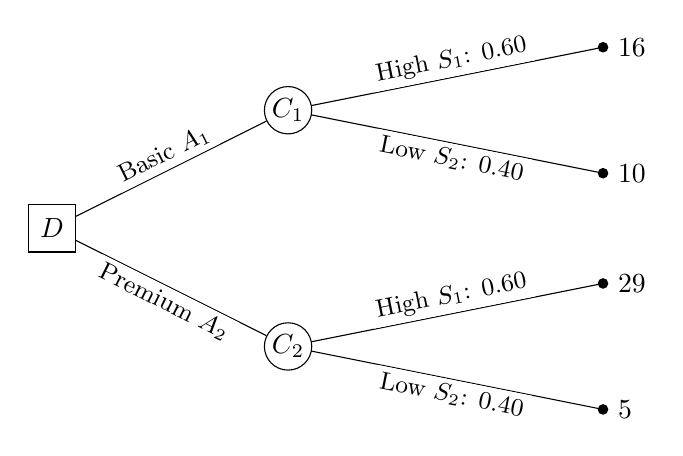
\begin{tikzpicture}[x=1cm,y=1cm]
\node[cNineDecision] (d) at (0,0) {$D$};
\node[cNineChance] (c1) at (3,1.5) {$C_1$};
\node[cNineChance] (c2) at (3,-1.5) {$C_2$};
\draw (d)--node[cNineLabel,above,sloped] {Basic $A_1$}(c1);
\draw (d)--node[cNineLabel,below,sloped] {Premium $A_2$}(c2);
\foreach \n/\yy/\pay in {1/2.3/16,2/0.7/10,3/-0.7/29,4/-2.3/5}{
\node[cNineEnd,label=right:{$\pay$}] (t\n) at (7,\yy) {};}
\draw (c1)--node[cNineLabel,above,sloped] {High $S_1$: $0.60$}(t1);
\draw (c1)--node[cNineLabel,below,sloped] {Low $S_2$: $0.40$}(t2);
\draw (c2)--node[cNineLabel,above,sloped] {High $S_1$: $0.60$}(t3);
\draw (c2)--node[cNineLabel,below,sloped] {Low $S_2$: $0.40$}(t4);
\end{tikzpicture}
\end{center}
Check: $0.60+0.40=1$ at \emph{each} circle. Keep this tree for Section~\ref{sec:solving}.
\secInicio[sec:booth][sec:building]

\subsection{Local Delivery Fleet (C9)}\label{sec:fleet}
A delivery firm chooses bicycles ($A_1$) or electric vans ($A_2$) before traffic is known. Clear traffic has probability $0.70$ and congestion $0.30$. Bicycles earn 4 thousand CNY per completed batch and complete 14 batches in clear traffic or 10 in congestion. Vans earn 6 thousand CNY per batch and complete 12 or 8 batches, respectively. Clear traffic adds a fixed bonus of 5 thousand CNY; congestion causes a fixed loss of 4 thousand CNY. No other costs apply.
\QuestionsTasks[sec:building]{
{9.3}/{task:fleet}/{Identify the node types and calculate all four terminal payoffs in thousand CNY. Then construct the labelled tree.}}
\phantomsection\label{task:fleet}
Use the earlier payoff convention:
\[
P_{ay}(A_i,S_j)=q(A_i,S_j)v^A(A_i)+f^S(S_j).
\]
Before drawing, organise your results in a two-alternative, two-state payoff table. Check that the decision occurs before traffic is observed. Leave space beside the circles for their EMVs.
\secInicio[sec:fleet][sec:building]

\subsection{Repair an Incorrect Tree (C9)}\label{sec:repair}
A greenhouse manager chooses a large or small greenhouse before the season is known. An excellent season has probability $0.30$, an average season $0.50$, and a poor season $0.20$. Large-greenhouse net profits are $70$, $30$, and $-10$; small-greenhouse net profits are $35$, $40$, and $32$.

A student draws a circle for the greenhouse choice, assigns probability $0.50$ to each greenhouse, and then draws squares for the seasons. The student omits the poor-season branch and writes $10$ instead of $-10$.
\QuestionsTasks[sec:building]{
{9.4}/{task:repair}/{Explain each error and draw the corrected tree, including all six terminal outcomes and the probability check at each chance node.}}
\phantomsection\label{task:repair}
\textbf{Self-check.} Which event can the manager choose? Can a loss be replaced by a positive profit? Does omitting an event leave the stated probabilities summing to one?
\secInicio[sec:repair][sec:building]

\section{Solving Decision Trees}\label{sec:solving}
\SectionProblemsTableOfContents{
\SectionProblemLink{sec:solve-booth}{4. Booth: Worked Backward Induction}\\
\SectionProblemLink{sec:solve-fleet}{5. Fleet and Greenhouse: Guided Practice}\\
\SectionProblemLink{sec:pilot}{6. Ferry Pilot: A Later Decision}}

\subsection{Booth: Worked Backward Induction (C9)}\label{sec:solve-booth}
\QuestionsTasks[sec:solving]{
{9.5}/{task:solve-booth}/{Value both chance nodes in the booth tree, then the initial decision node. Mark the selected branch and state the optimal strategy with its units.}}
\phantomsection\label{task:solve-booth}
\begin{align*}
V(C_1)=EMV(A_1)&=(0.60)(16)+(0.40)(10)=13.6,\\
V(C_2)=EMV(A_2)&=(0.60)(29)+(0.40)(5)=19.4,\\
V(D)&=\max\{13.6,19.4\}=19.4.
\end{align*}
Write $13.6$ and $19.4$ beside the circles and mark the premium branch at the square. The optimal strategy is to \textbf{choose the premium booth before attendance is known}, with expected net profit \$19,400. There is no later decision. The possible actual profits remain \$29,000 and \$5,000.
\secInicio[sec:solve-booth][sec:solving]

\subsection{Fleet and Greenhouse: Guided Practice (C9)}\label{sec:solve-fleet}
\QuestionsTasks[sec:solving]{
{9.6}/{task:solve-fleet}/{Solve your delivery-fleet tree. Show each EMV and the comparison at the square; state the chosen fleet and expected profit in thousand CNY.},
{9.7}/{task:solve-greenhouse}/{Solve the corrected greenhouse tree. Keep the negative payoff in your weighted average and explain the selected strategy.}}
\phantomsection\label{task:solve-fleet}
\textbf{Fleet scaffold.} Complete $EMV(A_1)=0.70(\ \ )+0.30(\ \ )$ and $EMV(A_2)=0.70(\ \ )+0.30(\ \ )$. Compare their values at the initial square.
\phantomsection\label{task:solve-greenhouse}
\textbf{Greenhouse scaffold.} For each circle, use all three season branches. Verify $0.30+0.50+0.20=1$ before calculating.
\secInicio[sec:solve-fleet][sec:solving]

\subsection{Ferry Pilot: A Later Decision (C9)}\label{sec:pilot}
A ferry operator can keep its current service for a certain net profit of $30$, or run a pilot. The pilot reveals strong demand with probability $0.60$ or weak demand with probability $0.40$. \emph{After observing demand}, the operator chooses whether to expand or retain the pilot service. With strong demand, expansion gives $75$ and retention $45$. With weak demand, expansion gives $10$ and retention $28$. These are total net profits, including the pilot cost. There is no further uncertainty.
\QuestionsTasks[sec:solving]{
{9.8}/{task:pilot-tree}/{Construct the tree: initial square, pilot circle, and one later square after each demand outcome. Label all five terminal payoffs.},
{9.9}/{task:pilot-solve}/{Solve the later squares first, then the pilot circle, then the initial square. State what to do after each observed demand outcome.}}
\phantomsection\label{task:pilot-tree}
\textbf{Timing guide.} The pilot branch has the sequence decision--chance--decision--terminal outcome. Keeping the current service leads directly to a terminal payoff.
\phantomsection\label{task:pilot-solve}
\textbf{Worked rollback.}
\[
V(D_{\mathrm{strong}})=\max\{75,45\}=75,\qquad
V(D_{\mathrm{weak}})=\max\{10,28\}=28.
\]
\[
V(C_{\mathrm{pilot}})=0.60(75)+0.40(28)=56.2,+\qquad V(D_0)=\max\{30,56.2\}=56.2.
\]
The optimal strategy is to \textbf{run the pilot; expand after strong demand and retain the pilot service after weak demand}. Expected net profit is \$56,200. Choosing expansion in both states would give only $0.60(75)+0.40(10)=49$.
\secInicio[sec:pilot][sec:solving]

\section{Mixed Contextual Practice}\label{sec:mixed}
\SectionProblemsTableOfContents{
\SectionProblemLink{sec:museum}{7. Museum Exhibition: Guided Multi-stage Tree}\\
\SectionProblemLink{sec:bike}{8. Electric-Bike Launch: Reduced Guidance}\\
\SectionProblemLink{sec:solar}{9. Solar Installer: Independent Practice}\\
\SectionProblemLink{sec:investment}{10. Business Investment: Independent Practice}}

\subsection{Museum Exhibition: Guided Multi-stage Tree (C9)}\label{sec:museum}
A museum chooses a compact exhibition for certain net profit $32$, or a trial exhibition. Trial attendance is high with probability $0.40$ and low with probability $0.60$. After seeing attendance, it chooses to keep the trial or extend it. Keeping yields $50$ after high attendance and $20$ after low attendance. Extending leads to uncertain sponsorship: after high attendance, sponsorship succeeds with probability $0.75$ and gives $90$, or fails with probability $0.25$ and gives $10$; after low attendance, success has probability $0.30$ and gives $55$, or failure has probability $0.70$ and gives $-5$. All payoffs are total net profits including trial and extension costs.
\QuestionsTasks[sec:mixed]{
{9.10}/{task:museum}/{Build and solve the full tree using the steps below. State the initial choice and the action after each attendance outcome.}}
\phantomsection\label{task:museum}
\begin{enumerate}
\item Begin with the compact/trial square. Add an attendance circle to the trial branch.
\item Put a keep/extend square after \emph{each} attendance outcome. Only extension branches lead to sponsorship circles. Use the probabilities conditional on that attendance outcome.
\item Label all seven terminal outcomes. Check every circle separately.
\item Calculate the two extension EMVs. Compare extension with keeping at each later square.
\item Weight the two selected continuation values by $0.40$ and $0.60$, then compare the trial value with $32$ at the initial square.
\end{enumerate}
\secInicio[sec:museum][sec:mixed]

\subsection{Electric-Bike Launch: Reduced Guidance (C9)}\label{sec:bike}
A retailer chooses a cautious launch for certain net profit $25$, or a market test costing $4$. The test reports favourable demand with probability $0.50$ and unfavourable demand with probability $0.50$. After observing the report, the retailer may stop or launch. Stopping generates no revenue and loses the test cost. If it launches, profits \emph{before deducting the test cost} are $90$ for high demand and $-10$ for low demand. After a favourable report, high/low probabilities are $0.80/0.20$; after an unfavourable report they are $0.25/0.75$. The cautious launch uses no test and its $25$ is already net.
\QuestionsTasks[sec:mixed]{
{9.11}/{task:bike}/{Build the complete tree, convert every tested-path payoff to net profit, and solve by backward induction. Annotate each node value and mark the optimal decisions. Write a strategy covering both reports.}}
\phantomsection\label{task:bike}
\textbf{Cost reminder.} Every path beginning with the test incurs $4$ once, even if the retailer stops. The later demand probabilities apply separately within each report branch.
\secInicio[sec:bike][sec:mixed]

\subsection{Solar Installer: Independent Practice (C9)}\label{sec:solar}
A solar installer chooses its current staffing plan for certain quarterly net profit $40$, or a training programme. Training succeeds with probability $0.70$ and fails with probability $0.30$. The result is observed before the next action. After success, the firm can serve local customers for certain profit $48$, or bid for a regional contract: winning has probability $0.60$ and gives $85$, while losing has probability $0.40$ and gives $15$. After failure, it can use a partner for certain profit $34$, or retrain: retraining succeeds with probability $0.50$ and gives $60$, or fails with probability $0.50$ and gives $0$. Every stated payoff is the total net profit including all training, bidding, or partnership costs along that path.
\QuestionsTasks[sec:mixed]{
{9.12}/{task:solar}/{Independently construct and solve the full tree. Show probability checks, terminal payoffs, all node values, and the optimal strategy with actions after both training outcomes.}}
\phantomsection\label{task:solar}
\secInicio[sec:solar][sec:mixed]

\subsection{Business Investment: Independent Practice (C9)}\label{sec:investment}
A small business can leave its funds in a deposit for certain net profit $12$, or invest in a delivery project. The first season is strong with probability $0.40$ or weak with probability $0.60$. After observing the season, it can sell the project or continue. Selling yields total net profit $35$ after a strong season or $5$ after a weak season. If it continues after a strong season, the second season is strong with probability $0.70$ or weak with probability $0.30$, giving total net profits $65$ or $15$. If it continues after a weak first season, the second season is strong with probability $0.20$ or weak with probability $0.80$, giving total net profits $30$ or $-10$. All final payoffs include both seasons and all project costs; do not add a separate first-season profit.
\QuestionsTasks[sec:mixed]{
{9.13}/{task:investment}/{Build and solve the tree without a scaffold. Explain why the continuation probabilities differ between the two first-season outcomes. State the full optimal strategy and its expected net profit.}}
\phantomsection\label{task:investment}
\textbf{Final review.} Does your tree respect the timing? Are choices squares and uncertainties circles? Does each circle have a complete probability distribution? Have you used net payoffs, weighted averages at circles, and maxima at squares? Does your strategy specify later actions rather than only an initial choice?
\secInicio[sec:investment][sec:mixed]

\subsection*{Check your results after completing the practice}
These checkpoints support self-assessment; a complete answer still requires the labelled tree and backward-induction calculations.
\begin{itemize}
\item \textbf{Fleet:} payoffs $61,36$ for bicycles and $77,44$ for vans. EMVs are $53.5$ and $67.1$ thousand CNY; choose vans.
\item \textbf{Greenhouse:} large EMV $=34$; small EMV $=36.9$. Choose small.
\item \textbf{Museum:} extension EMVs $70$ after high attendance and $13$ after low attendance. Extend after high; keep after low. Trial EMV $=0.40(70)+0.60(20)=40$; choose trial over compact ($32$).
\item \textbf{Electric bikes:} tested-path payoffs are $86,-14$ if launching and $-4$ if stopping. Launch EMVs are $66$ after favourable and $11$ after unfavourable reports, both better than stopping. Test EMV $=38.5$; choose the test and launch after either report.
\item \textbf{Solar:} regional-bid EMV $=57$; retraining EMV $=30$. After success bid; after failure use a partner. Training EMV $=0.70(57)+0.30(34)=50.1$; choose training.
\item \textbf{Investment:} continuation EMVs are $50$ after a strong first season and $-2$ after a weak first season. Continue after strong; sell after weak. Project EMV $=0.40(50)+0.60(5)=23$; invest rather than take the deposit ($12$).
\end{itemize}
\end{document}
